\chapter{Implementation}
Implementation was done using the Google Colaboratory. All the modifications that I've done to the original template are accompanied by the comments that I've put.

Below, I've added additional explanations for some of the features that I've used or modified.


\section{Initialization}

I have initialized some boolean parameters to be used later on for the training/evaluation/testing.

\begin{figure}[htbp]
\centering
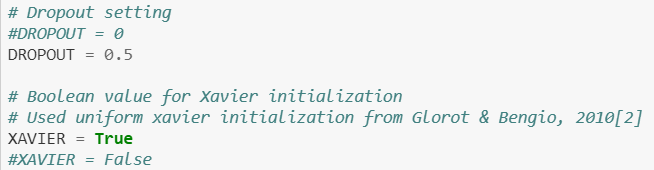
\includegraphics[width=0.6\linewidth]{implementation/fig/code0.png}
\caption{Initialization}
\label{fig:code0}
\end{figure}

\section{TensorBoardColab}

{\bf TensorBoard} is a visualization toolkit that supports various experimentation. Especially, it is useful in tracking and visualizing metrics such as loss and accuracy.

It is supported in multiple platforms, including Tensorflow, Google Colaboratory...etc.

\begin{figure}[htbp]
\centering
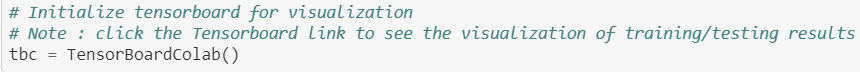
\includegraphics[width=0.6\linewidth]{implementation/fig/code1.png}
\caption{TensorBoardColab}
\label{fig:code1}
\end{figure}


\section{GraphConvolutionLayer}

\subsection{Parameter Initialization}

Here I have given myself two choices for initializing weights:
\begin{enumerate}
\item Sampling from $U \left(-\frac{1}{\sqrt{m}}, \frac{1}{\sqrt{m}}\right)$\cite{Goodfellow2016}
\item Xavier initialization\cite{Glorot2010}
\end{enumerate}

For either case, bias was initialized by sampling from $U \left(-\frac{1}{\sqrt{m}}, \frac{1}{\sqrt{m}}\right)$.

\begin{figure}[htbp]
\centering
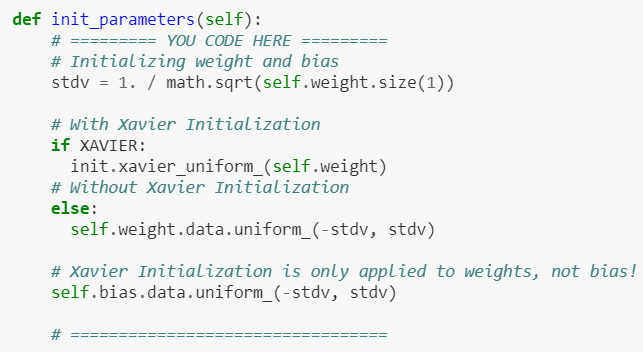
\includegraphics[width=0.6\linewidth]{implementation/fig/code2.png}
\caption{Parameter initialization}
\label{fig:code2}
\end{figure}

\subsection{Forward Function}

For forward propagation, I have used the heuristic of
$$forward(H) = A H W + b$$
where $A$ is the adjacency matrix, $H$ is the input matrix, $W$ is the weight matrix, and $b$ is the bias matrix.

\begin{figure}[htbp]
\centering
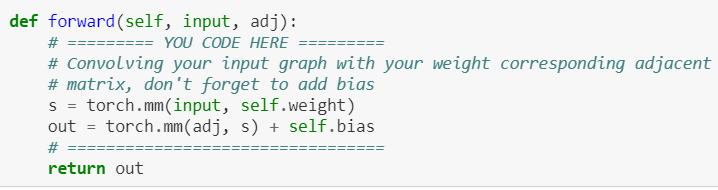
\includegraphics[width=0.6\linewidth]{implementation/fig/code3.png}
\caption{Forward propagation}
\label{fig:code3}
\end{figure}

\section{GCN}

\subsection{Network Initialization}

Following the work of Kipf \& Welling\cite{Kipf2017}, I have decided to implemented the two-layered GCN. To do that, two {\it GraphConvolutionLayer}'s, along with {\it dropout}, were initialized.

\begin{figure}[htbp]
\centering
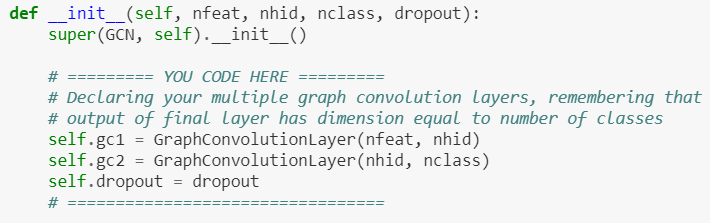
\includegraphics[width=0.6\linewidth]{implementation/fig/code4.png}
\caption{Network initialization}
\label{fig:code4}
\end{figure}

\subsection{Forward Function}

I have used the forward model of the form:
$$forward(X, A) = \softmax\left(\hat{A}  \relu\left( \hat{A} X W^{(0)} \right) W^{(1)} \right)$$

\begin{figure}[htbp]
\centering
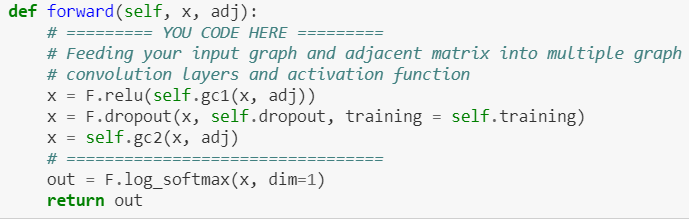
\includegraphics[width=0.6\linewidth]{implementation/fig/code5.png}
\caption{Forward propagation}
\label{fig:code5}
\end{figure}

\section{Training/Validation/Testing}

(Even though I only describe one of the three here, the rest are the same. Just change the index set to the appropriate one.)

I have utilized the negative log likelihood loss. Also, I have updated the tensorboard plot for every epoch.

\begin{figure}[htbp]
\centering
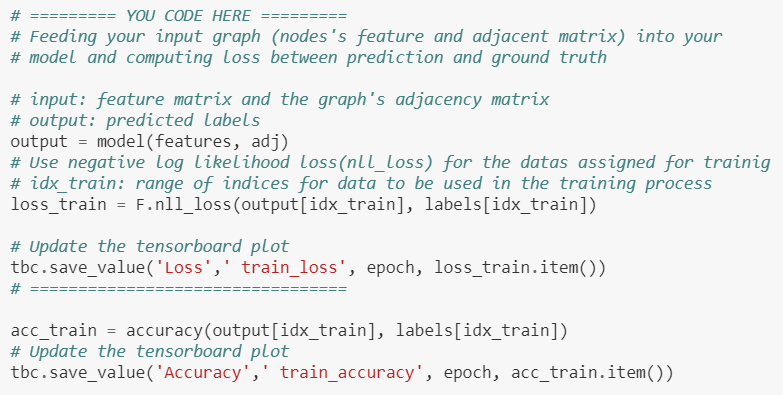
\includegraphics[width=0.6\linewidth]{implementation/fig/code6.png}
\caption{Training phase}
\label{fig:code6}
\end{figure}

\section{Confusion Matrix}

For the confusion matrix plot, I have utilized the external github open repository: \url{https://github.com/wcipriano/pretty-print-confusion-matrix}.

\begin{figure}[htbp]
\centering
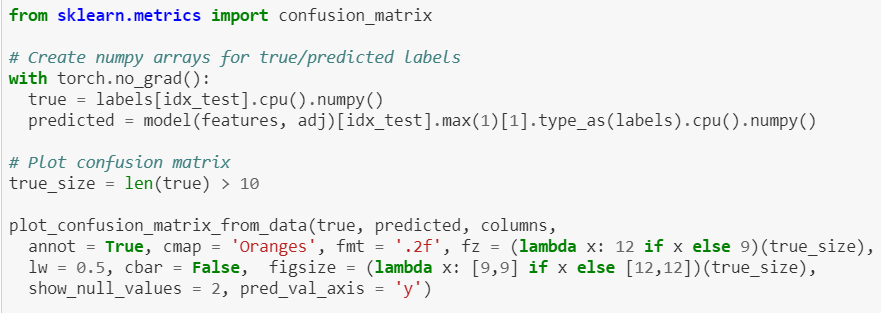
\includegraphics[width=0.6\linewidth]{implementation/fig/code7.png}
\caption{Confusion matrix}
\label{fig:code7}
\end{figure}